% =====================================================================
%  Task 1 - Reinforcement Learning  (Bericht)
%  Kompilieren:  pdflatex Task1_Report.tex
%  Diese Datei ist bewusst einfach gehalten, damit sie leicht
%  selbst weiter bearbeitet werden kann.
% =====================================================================
\documentclass[11pt,a4paper]{article}

\usepackage[T1]{fontenc}
\usepackage[utf8]{inputenc}
\usepackage[ngerman]{babel}
\usepackage{amsmath,amssymb}
\usepackage[a4paper,margin=2.3cm]{geometry}
\usepackage{graphicx}
\usepackage{booktabs}
\usepackage{xcolor}
\usepackage{enumitem}
\usepackage{titlesec}
\usepackage[hidelinks]{hyperref}
\usepackage[backend=biber, style=authoryear]{biblatex}
\addbibresource{references.bib}

% --- einfache Farben / Ueberschriften im Stil des Task-2-Berichts ---
\definecolor{headblue}{RGB}{47,84,150}
\titleformat{\section}{\color{headblue}\large\bfseries}{\thesection.}{0.5em}{}
\titleformat{\subsection}{\color{black!75}\normalsize\bfseries}{\thesubsection}{0.5em}{}
\titlespacing{\section}{0pt}{10pt}{4pt}
\setlist[itemize]{topsep=2pt,itemsep=2pt,parsep=0pt,leftmargin=1.4em}

\setlength{\parindent}{0pt}
\setlength{\parskip}{5pt}

% --- Titel ---
\title{\vspace{-1.2cm}\bfseries\color{black}
       L\"osung von SeaShanty mit tabularem Reinforcement Learning}
\author{}
\date{}

\begin{document}
\maketitle
\vspace{-2.2cm}
{\color{black!60}Task 1 -- Reinforcement Learning (Prof.\ Thomas Nierhoff, OTH Amberg-Weiden)\\
Autor: Himanshu Mohan Nikam}
\vspace{6pt}

% =====================================================================
\section{Projekt\"uberblick}
% =====================================================================
Ziel von Task~1 ist es, die Umgebung \texttt{SeaShanty(size=12, period=6)} mit
\emph{m\"oglichst wenigen Episoden} zu l\"osen. Der Agent bewegt sich auf einem
$12\times12$-Gitter, in dem sich t\"odliche \glqq Wasser\grqq{}-Zellen in jedem Schritt
nach einem festen Muster bewegen. Der Agent bekommt $+100$ f\"ur das Ziel,
$-100$ f\"ur Wasser und $0$ sonst. Da sich das Wasser mit dem Schritt-Z\"ahler $t$
bewegt und \texttt{reset()} $t$ zu Beginn jeder Episode auf $0$ setzt, ist dieselbe
Zelle mal sicher und mal t\"odlich.

Das Projekt besteht aus mehreren eigenen Dateien. Die vorgegebenen Dateien
(\texttt{gridworld.py}, \texttt{plot.py}, \texttt{config.py}) wurden nicht ver\"andert:
\begin{itemize}
  \item \texttt{task1.py} -- Q-Learning und Double Q-Learning, plus die geforderte
        Lernkurve und die Q-/V-Tabellen-Plots.
  \item \texttt{sarsa.py} -- SARSA und n-step SARSA.
  \item \texttt{tune.py} -- Optuna-Tuning f\"ur die Methoden in \texttt{task1.py}.
  \item \texttt{sarsa\_tune.py} -- Optuna-Tuning f\"ur die Methoden in \texttt{sarsa.py}.
\end{itemize}

Gemessen wird die \glqq reale\grqq{} kumulierte Belohnung pro Episode (die Summe der
echten, \emph{nicht} geshapten Belohnungen), gemittelt \"uber 100 verschiedene
Umgebungen (Seeds 1000--1099). F\"ur das Tuning werden andere Seeds (0--29) benutzt
als f\"ur die finale Auswertung.

% =====================================================================
\section{Ans\"atze}
% =====================================================================
\subsection{Wertbasiert: Q-Learning (in task1.py)}
Q-Learning lernt direkt die optimale Aktions-Bewertung $Q(s,a)$. Zus\"atzlich haben
wir \textbf{Double Q-Learning} umgesetzt: Es benutzt zwei Tabellen und trennt die
Auswahl der Aktion von ihrer Bewertung, um die \"Ubersch\"atzung der Werte zu
reduzieren -- das ist neben der gro\ss en $-100$-Strafe besonders wichtig.

\subsection{On-policy: SARSA (in sarsa.py)}
SARSA bewertet die Politik, der es wirklich folgt, und ist dadurch \emph{vorsichtiger}
nahe am t\"odlichen Wasser. Wir haben \textbf{SARSA}, \textbf{Expected SARSA} und
\textbf{n-step SARSA} ($n=4$) umgesetzt. Expected SARSA bootstrappt auf dem Erwartungswert
$E_\pi[Q(s',a')]$ statt auf einer einzelnen n\"achsten Aktion (geringere Varianz); n-step
gibt die Belohnungs-Information mehrere Schritte weiter zur\"uck und verteilt so das Lob
schneller entlang des Weges zum Ziel.

% =====================================================================
\section{Wichtige Techniken}
% =====================================================================
\begin{itemize}
  \item \textbf{Phase Augmentation.} Reines positionsbasiertes Q-Learning verletzt
        die Markov-Eigenschaft, weil sich das Wasser mit $t$ bewegt; so l\"ost es nur
        etwa 10\,\% der Umgebungen. Wir erweitern den Zustand um die Phase:
        \texttt{state = position*K + (t mod K)} mit $K=38 \approx \mathrm{round}(2\pi\cdot period)$.
        Da jeder L\"osungsweg k\"urzer als $K$ Schritte ist, gilt $t \bmod K = t$, und
        der Zustand wird wieder Markov.
  \item \textbf{Potential-based Reward Shaping.} Bei Schrittkosten $0$ ist die
        Belohnung sehr d\"unn. Wir addieren $F = \gamma\,\Phi(s') - \Phi(s)$
        (Ng et al., 1999) mit $\Phi = -(\text{Manhattan-Distanz zum Ziel})$, normiert
        und mit einem Gewicht \texttt{SHAPE\_W} skaliert. Das ist policy-invariant,
        ver\"andert also die optimale Politik nicht, sondern lenkt nur das Lernen.
        Die reale Belohnung enth\"alt $F$ nie.
  \item \textbf{Optimistische Initialisierung.} Ein optimistischer Q-Startwert bringt
        die Greedy-Politik dazu, systematisch neue Aktionen zu probieren -- \emph{ohne}
        die Zufalls-Tode, die eine hohe Epsilon-Schwelle in dieser t\"odlichen Umgebung
        verursachen w\"urde.
\end{itemize}

% =====================================================================
\section{Versuchsaufbau}
% =====================================================================
Alle Agenten sind einfache NumPy-Tabellen. Die Hyperparameter ($\gamma$, $\alpha$,
Epsilon-Start, Epsilon-Decay, optimistischer Startwert, Shaping-Gewicht und $n$ f\"ur
n-step SARSA) werden mit \textbf{Optuna} gesucht (50 Trials pro Methode). Die
Tuning-Seeds (0--29) sind von den Auswertungs-Seeds (1000--1099) getrennt. Das
Tuning-Ziel maximiert die mittlere reale Belohnung \"uber alle Episoden und belohnt
so \emph{schnelles} Lernen.

% =====================================================================
\section{Ergebnisse}
% =====================================================================
Abbildung~\ref{fig:compare} zeigt das zentrale Ergebnis: die reale kumulierte Belohnung
pro Episode, gemittelt \"uber 100 Umgebungen (Seeds 1000--1099), f\"ur alle f\"unf Methoden.
Jede Methode benutzt ihre \emph{eigenen} mit Optuna getunten Hyperparameter; die orange
Q-Learning-Kurve ist zugleich die geforderte Lernkurve (Summe der echten, nicht geshapten
Belohnungen).

Q-Learning, 1-Schritt-SARSA und Expected SARSA steigen z\"ugig auf etwa $+95$ und l\"osen
die Umgebung nach rund 100--120 Episoden. Double Q-Learning und n-step SARSA lernen deutlich
langsamer: Ihre Kurven steigen zwar stetig, erreichen innerhalb von 300 Episoden aber nur
die \glqq \"Uberlebens\grqq-Politik um $0$ und noch nicht das Ziel (Gr\"unde siehe
Diskussion). Expected SARSA verh\"alt sich praktisch wie 1-Schritt-SARSA -- sein Vorteil,
die geringere Varianz durch den Erwartungswert statt einer einzelnen Stichprobe, wirkt vor
allem in \emph{stochastischen} Umgebungen; hier ist die Dynamik pro Episode deterministisch,
daher der kaum sichtbare Unterschied.

\IfFileExists{methods_comparison.png}{%
\begin{figure}[h]
  \centering
  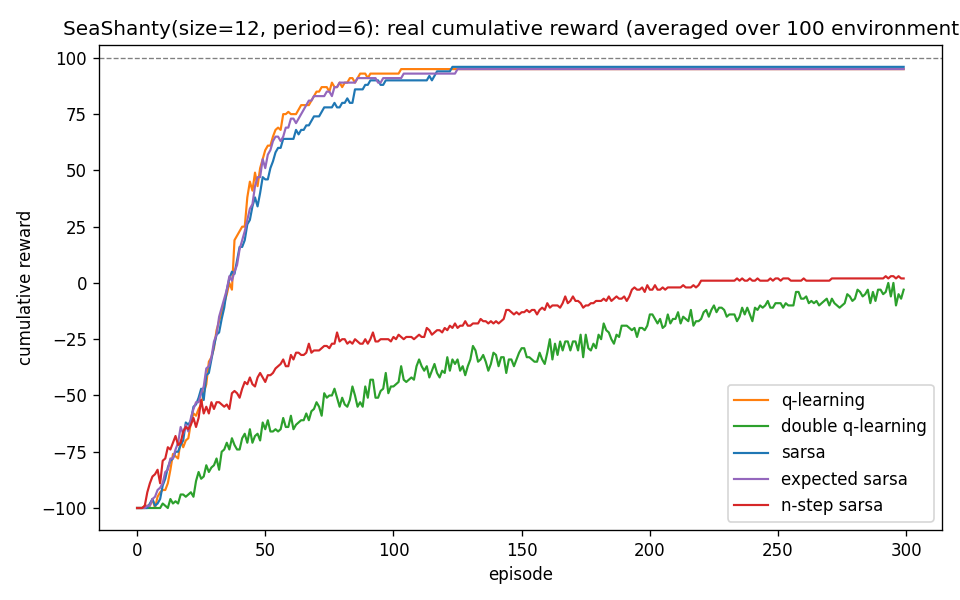
\includegraphics[width=0.68\textwidth]{methods_comparison.png}
  \caption{Vergleich aller f\"unf Methoden: reale kumulierte Belohnung pro Episode,
           gemittelt \"uber 100 Umgebungen (Seeds 1000--1099), jede mit ihren \emph{eigenen}
           getunten Hyperparametern. Die Q-Learning-Kurve ist die geforderte Lernkurve.}
  \label{fig:compare}
\end{figure}}{}

\begin{table}[h]
\centering
\small
\begin{tabular}{@{}llll@{}}
\toprule
\textbf{Methode} & \textbf{Verhalten} & \textbf{Reale Belohnung (Ep 300)} & \textbf{Anmerkung}\\
\midrule
Q-Learning        & l\"ost schnell & $\rightarrow +95$ & prim\"are L\"osung, am schnellsten\\
SARSA (1-Schritt) & l\"ost schnell & $\rightarrow +95$ & fast so schnell wie Q-Learning\\
Expected SARSA    & l\"ost schnell & $\rightarrow +95$ & wie SARSA, geringere Varianz\\
Double Q-Learning & \"uberlebt     & $\approx 0$ & konvergiert langsam (zwei Tabellen)\\
n-step SARSA ($n{=}4$) & \"uberlebt & $\approx 0$ & konvergiert langsam (n-step-Returns)\\
\bottomrule
\end{tabular}
\caption{Vergleich der Methoden auf den Auswertungs-Umgebungen (Seeds 1000--1099) nach
         300 Episoden, jede mit ihren \emph{eigenen} getunten Hyperparametern.
         Q-Learning, 1-Schritt-SARSA und Expected SARSA l\"osen; Double Q-Learning und
         n-step SARSA erreichen nur die \"Uberlebens-Politik ($\approx 0$).}
\end{table}

% =====================================================================
\section{Fehlgeschlagene Versuche}
% =====================================================================
Wir berichten bewusst auch, was \emph{nicht} funktioniert hat.

\subsection{Reward Shaping ohne Skalierung}
Ohne die Skalierung mit \texttt{SHAPE\_W} bleibt das Potential im Bereich $[0,1]$; die
Steigung ist dann nur etwa $1/22 \approx 0{,}045$ pro Schritt und damit viel zu klein
gegen\"uber den $\pm100$ der Endzust\"ande. Das haben wir f\"ur beide Familien
getestet:
\begin{itemize}
  \item \textbf{SARSA / n-step SARSA:} Die Kurve bleibt bei etwa $0$ stehen -- der
        Agent \glqq \"uberlebt\grqq{} nur und meidet das Wasser -- und erreicht das
        Ziel nur selten; rund 10\,\% der Umgebungen werden gel\"ost.
  \item \textbf{Q-Learning / Double Q-Learning} (auf einem anderen Rechner getunt,
        siehe \texttt{qlearning\_without\_scaling\_tuning.txt}): Das Ergebnis ist stark
        verrauscht -- etwa 42\,\% der Umgebungen gel\"ost, aber viele Tode. Die
        gemittelte Kurve steht bei Episode~199 noch bei $-10$. Selbst nach 50
        Optuna-Trials war der beste Tuning-Wert nur $-96{,}7$ (Q-Learning) bzw.
        $-3{,}4$ (Double Q-Learning) -- ein deutliches Zeichen, dass fast nichts gelernt
        wurde.
\end{itemize}
Mit Skalierung (\texttt{SHAPE\_W} $\approx 80$--$125$) erreicht Q-Learning das Ziel
dagegen zuverl\"assig, und die Kurve steigt schon nach etwa 125--150 Episoden auf
$+100$. Das Skalieren des Potentials ist policy-invariant (nur die Lerngeschwindigkeit
\"andert sich, nicht die optimale Politik) und war hier der entscheidende Schritt.

\subsection{Weitere gescheiterte Ideen}
\begin{itemize}
  \item \textbf{Hohe Epsilon-Schwelle zur Exploration:} fatal. Zuf\"allige Wege sterben
        im t\"odlichen Wasser, bevor sie das Ziel finden. Die Exploration muss
        stattdessen von der geshapten, optimistischen Greedy-Politik kommen.
  \item \textbf{Nur Phase Augmentation ohne Shaping:} l\"ost die Umgebung zwar, braucht
        aber \"uber 4000 Episoden.
  \item \textbf{Tuning auf schwachem (un-skaliertem) Shaping:} liefert fast kein Signal
        (fast alle Trials $\approx -99$), also praktisch zuf\"allige Hyperparameter.
        Werden diese sp\"ater mit skaliertem Shaping benutzt, sind die Ergebnisse
        schlechter als beim Original. Das Tuning sollte immer mit dem \emph{skalierten}
        Shaping laufen.
\end{itemize}

% =====================================================================
\section{Diskussion}
% =====================================================================
Die gr\"o\ss te Schwierigkeit ist die Nicht-Stationarit\"at der Umgebung, nicht die
Lernregel. Mit Phase Augmentation wird das Problem Markov, und Off-policy-Q-Learning
l\"ost es zuverl\"assig; ohne Augmentation hilft kein Tuning.

Interessant ist, dass mit \emph{skaliertem} Reward Shaping und getunten Hyperparametern
nicht nur das off-policy Q-Learning, sondern auch das on-policy \mbox{1-Schritt-SARSA}
die Aufgabe zuverl\"assig und etwa gleich schnell l\"ost (Abbildung~\ref{fig:compare}).
Das starke Shaping-Signal \"uberwiegt hier die sonst typische Vorsicht von SARSA. Ohne
Skalierung (Abschnitt~6) bleibt SARSA dagegen bei der reinen \glqq \"Uberlebens\grqq-Politik
bei Belohnung~$0$ stehen -- entscheidend ist also das Shaping, nicht die Wahl von on-
gegen off-policy.

Die beiden langsameren Methoden -- \textbf{Double Q-Learning} und \textbf{n-step SARSA}
-- wurden hier bewusst mit ihren \emph{eigenen} getunten Hyperparametern ausgewertet und
bleiben trotzdem innerhalb von 300 Episoden bei der \"Uberlebens-Politik (Belohnung um
$0$). Ihre zus\"atzliche Maschinerie bremst das Lernen in dieser Aufgabe eher, als dass
sie hilft: Double Q-Learning verteilt die Updates auf zwei Tabellen und halbiert so
praktisch die effektive Lernrate pro Tabelle, und die n-step-Returns machen die Updates
verrauschter. Beide Kurven steigen jedoch stetig weiter und w\"urden mit mehr Episoden
voraussichtlich ebenfalls das Ziel erreichen. Bemerkenswert ist, dass die Trennung nicht
entlang on-/off-policy verl\"auft -- je eine Methode aus beiden Lagern l\"ost, je eine
\"uberlebt nur --, sondern entlang der Komplexit\"at der Lernregel.

% =====================================================================
\section{Fazit}
% =====================================================================
Wir haben zwei Familien tabularer Agenten verglichen -- Q-Learning/Double Q-Learning
und SARSA/n-step SARSA -- zusammen mit Phase Augmentation, skaliertem Reward Shaping und
optimistischer Initialisierung. Phase-augmentiertes Q-Learning ist der schnellste und
zuverl\"assigste Ansatz und bringt die mittlere reale Belohnung in etwa 100--120 Episoden
auf $+95$; mit skaliertem Shaping l\"ost auch 1-Schritt-SARSA die Aufgabe \"ahnlich
schnell, w\"ahrend Double Q-Learning und n-step SARSA -- selbst mit eigenem Tuning --
innerhalb von 300 Episoden nur die \"Uberlebens-Politik erreichen und mehr Episoden
ben\"otigen. Ohne die Skalierung des Shaping-Potentials scheitern dagegen alle Methoden,
wie die dokumentierten Versuche zeigen.

\newpage
\section{Quellen}
\nocite{*}
\printbibliography

\end{document}
